\documentclass[a4paper,12pt]{article}
\usepackage[utf8]{inputenc}
\usepackage[italian]{babel}
\usepackage{amsfonts}
\usepackage{listings}
\usepackage{xcolor}
\usepackage{booktabs}
\usepackage{graphicx}
\usepackage{float}
\setcounter{tocdepth}{4}
\setcounter{secnumdepth}{4}

\title{Red-Black Trees}
\author{Appunti di Programmazione}
\date{\today}

\begin{document}
\tableofcontents
\newpage

\maketitle

\section{Red-Black Trees}

Un Red-Black Tree è un albero di ricerca binario (BST) bilanciato in cui ogni nodo ha un attributo extra: il \textbf{colore}, che può essere rosso o nero.

\subsection{Proprietà Fondamentali}
Per essere un Red-Black Tree valido, devono essere soddisfatte le seguenti proprietà:
\begin{enumerate}
    \item Ogni nodo è o rosso o nero.
    \item La radice è sempre nera.
    \item Le foglie (NIL) sono considerate nere.
    \item Se un nodo è rosso, entrambi i suoi figli devono essere neri (non possono esserci due nodi rossi consecutivi).
    \item Per ogni nodo, tutti i cammini semplici dal nodo alle foglie discendenti contengono lo stesso numero di nodi neri (proprietà della \textit{black-height}).
\end{enumerate}
\begin{figure}[H]
    \centering
    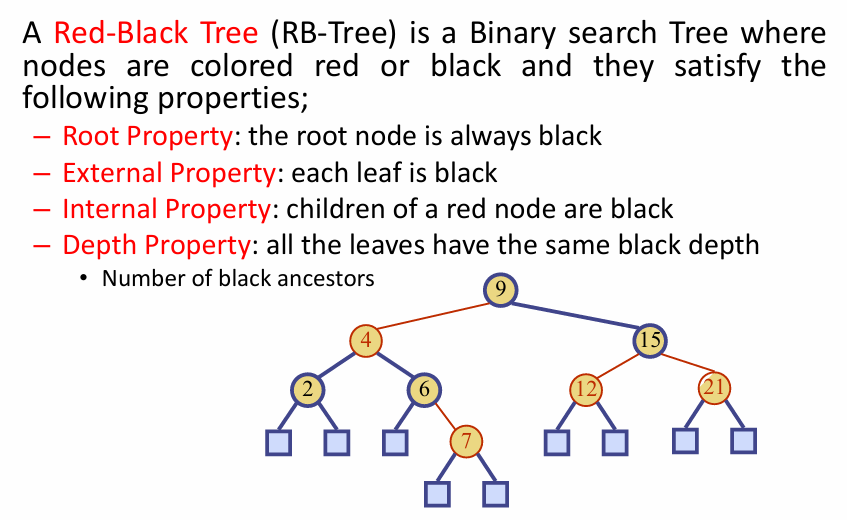
\includegraphics[width=0.6\linewidth]{Immagini/RedBlackDef.png}
    \caption{Proprietà di un Red-Black Tree}
\end{figure}



\subsection{Relazione con gli (2,4)-Trees}
Esiste una corrispondenza strutturale tra Red-Black Trees e (2,4)-trees (un tipo di a-b tree). 
Un nodo nero in un RB-Tree, insieme ai suoi eventuali figli rossi, può essere visto come un singolo nodo di un (2,4)-tree:
\begin{itemize}
    \item Un nodo nero senza figli rossi $\rightarrow$ nodo con 1 chiave (2 figli).
    \item Un nodo nero con 1 figlio rosso $\rightarrow$ nodo con 2 chiavi (3 figli).
    \item Un nodo nero con 2 figli rossi $\rightarrow$ nodo con 3 chiavi (4 figli).
\end{itemize}

\begin{figure}[H]
    \centering
    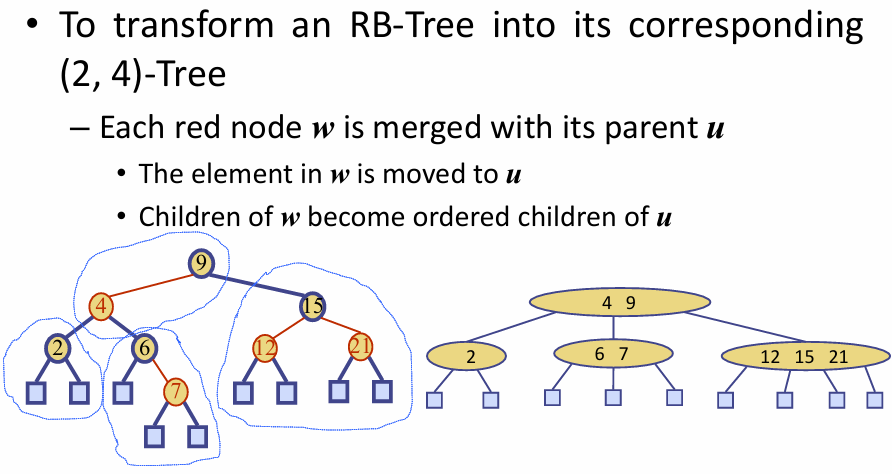
\includegraphics[width=0.48\linewidth]{Immagini/RedBlack24.png}
    \vline
    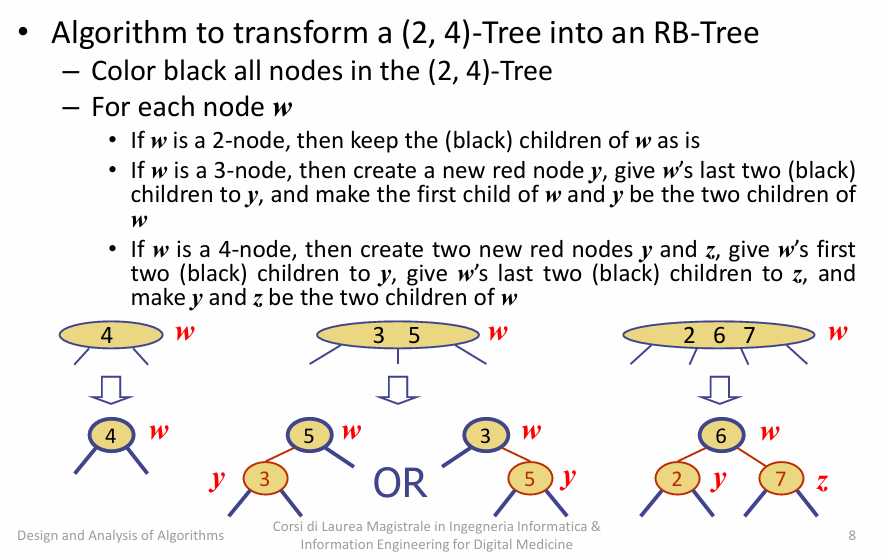
\includegraphics[width=0.48\linewidth]{Immagini/24RedBlack.png}
    \caption{Corrispondenza tra Red-Black Trees e (2,4)-trees}
\end{figure}

\subsection{Inserimento in un Red-Black Tree}
L'inserimento in un Red-Black Tree segue le stesse regole di inserimento di un BST, ma dopo l'inserimento è necessario eseguire alcune operazioni per mantenere le proprietà del Red-Black Tree.
\begin{figure}[H]
    \centering
    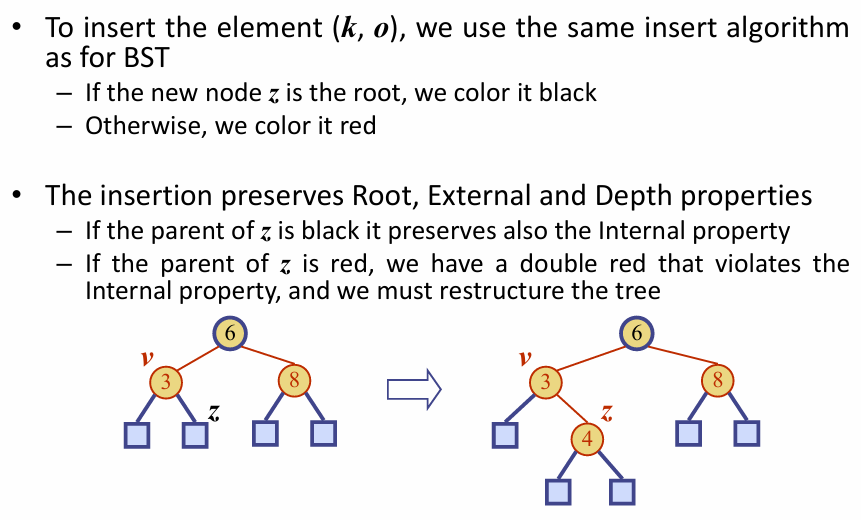
\includegraphics[width=0.6\linewidth]{Immagini/RedBlackInsert.png}
    \caption{inserimento in un Red-Black Tree}
\end{figure}
Il nodo da inserire si colora sempre di rosso, se è la radice allora di nero. 
Se il padre del nodo inserito è nero, non è necessario fare nulla. Se il padre è rosso, si devono eseguire delle rotazioni e/o cambi di colore 
per mantenere le proprietà del Red-Black Tree (il padre di un nodo rosso è sempre nero).




\end{document}